% Copyright: CSCE240-001 - Fall 2016 - Group 7. All rights reserved.
% Date: 2016-11-30
%
% This traces the execution

\chapter{Execution Trace}

The execution begins at an entry point referred to here as \texttt{Main} and procedes, most distally, to \texttt{OneVoter} through a topology described in Figure~\ref{hxtk-exec-topology}.

Execution begins at \texttt{Main}. First, all variables used by \texttt{Main} are declared. First, boilerplate program entry is taken care of: Arguments are validated, files are opened, system state is recorded, etc.

An instance of \texttt{Configuration} is initialized from the corresponding stream, which is then closed.

\section{Configuration}

\texttt{Configuration} is a \emph{Singleton} collection of public variables that will be used throughout the program. It accepts an open stream for the configuration file, which should be of the format described in \S\ref{hxtk-config-file}. Next, a log-normal data set is read in by the same call. This stream is opened in context by the \texttt{Configuration::ReadConfiguration} function. \emph{NOTE: The program will crash if the file is not found.} The conditions for this file are given in \S\ref{hxtk-data-file}.

From here, execution returns to \texttt{Main} and procedes to \texttt{Simulation}.

\section{Simulation}

Simulation does very little work and exists only to group \texttt{Precinct}s into batches. Precincts are read in from a file first, then execution is passed off to each precinct in turn to run its simulation.

\section{OnePct}

This is the ``meat'' of the program. Execution first enters \texttt{OnePct} at \texttt{RunSimulationPct}.

A simulation runs through a day of voting in order to determine the number of voting booths required to handle voters efficiently. The purpose of \texttt{OnePct::RunSimulationPct} is to regulate the number of voting booths being simulated. Given a mean voting time in seconds ($MVT$) and a number of voters ($NV$) on an election day ($L$) hours long, the initial number of voting booths ($VB_0$) is given by Equation~\ref{hxtk-init-booths} below.

\begin{equation} \label{hxtk-init-booths}
VB_0 = \begin{cases}
  \lfloor \frac{MVT \times NV}{3600\times L} \rfloor & MVT \times NV \ge 3600\times L \\
  1 & \text{otherwise}
\end{cases}
\end{equation}

Beginning with this number and iterating upwards until no voters are waiting ``too long,'' the program runs the number of iterations indicated by \S\ref{hxtk-config-file}. After all iterations have run, a histogram is printed if this number of voting machines is a breakpoint number for this precinct.

\subsection{CreateVoters}

Each single iteration consists of three parts. First, voters are created. This includes a set of voters waiting at the door when the polls open and exponential random voters at the hourly rates indicated by the configuration file.

\subsection{RunSimulationPct2}

Next, simulation is passed off to another function. This manages the processing of voters through the queue.

\subsection{DoStatistics}

Finally, some statistics are run to determine if any voters waited too long, among other things.

\begin{figure}
\begin{center}
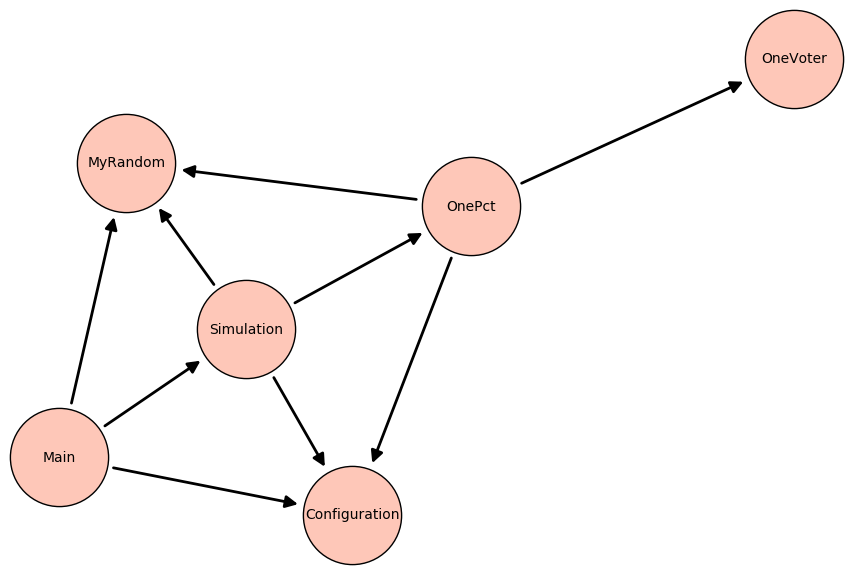
\includegraphics[width=\textwidth]{execution_topology}
\end{center}
\caption{Execution Topology by Class} \label{hxtk-exec-topology}
\end{figure}